\documentclass[border=6pt]{standalone}
\usepackage{tikz}
\usetikzlibrary{arrows.meta,positioning,shapes.geometric}
\begin{document}
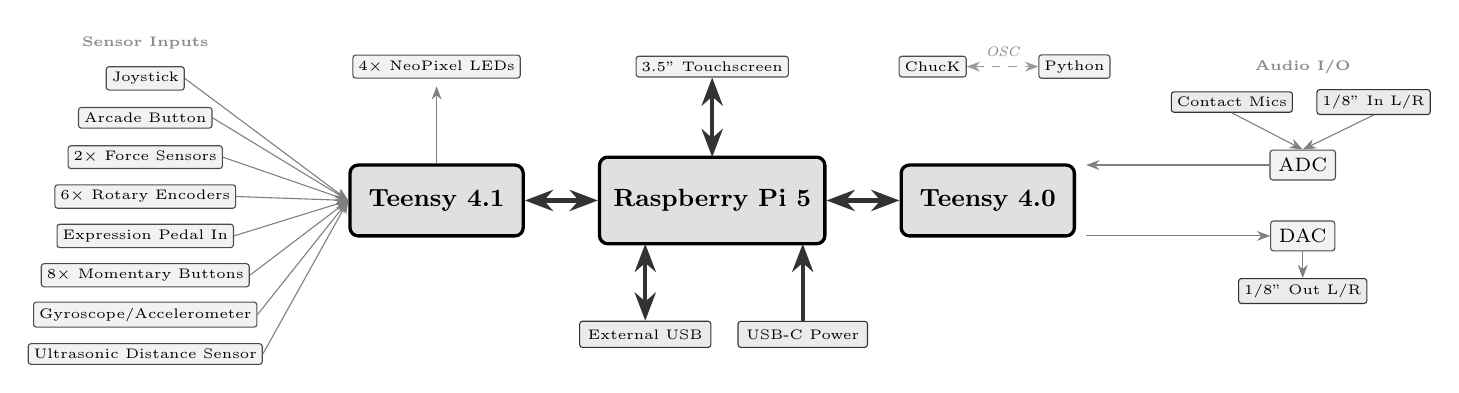
\begin{tikzpicture}

% === THREE PLATFORMS ===
\node[rectangle, draw=black, very thick, fill=black!12, rounded corners=3pt, font=\small\bfseries, inner sep=5pt, minimum height=1.1cm, minimum width=2.6cm] (pi) at (0,0) {Raspberry Pi 5};
\node[rectangle, draw=black, very thick, fill=black!12, rounded corners=3pt, font=\small\bfseries, inner sep=4pt, minimum height=0.9cm, minimum width=2.2cm] (t41) at (-3.5,0) {Teensy 4.1};
\node[rectangle, draw=black, very thick, fill=black!12, rounded corners=3pt, font=\small\bfseries, inner sep=4pt, minimum height=0.9cm, minimum width=2.2cm] (t40) at (3.5,0) {Teensy 4.0};

\draw[Stealth-Stealth, line width=1.6pt, black!80] (t41.east) -- (pi.west);
\draw[Stealth-Stealth, line width=1.6pt, black!80] (t40.west) -- (pi.east);

% === SENSORS ===
\node[rectangle, draw=black!70, fill=black!5, rounded corners=1pt, font=\tiny, inner sep=2pt] (s1) at (-7.2, 1.55) {Joystick};
\node[rectangle, draw=black!70, fill=black!5, rounded corners=1pt, font=\tiny, inner sep=2pt] (s2) at (-7.2, 1.05) {Arcade Button};
\node[rectangle, draw=black!70, fill=black!5, rounded corners=1pt, font=\tiny, inner sep=2pt] (s3) at (-7.2, 0.55) {2$\times$ Force Sensors};
\node[rectangle, draw=black!70, fill=black!5, rounded corners=1pt, font=\tiny, inner sep=2pt] (s4) at (-7.2, 0.05) {6$\times$ Rotary Encoders};
\node[rectangle, draw=black!70, fill=black!5, rounded corners=1pt, font=\tiny, inner sep=2pt] (s5) at (-7.2,-0.45) {Expression Pedal In};
\node[rectangle, draw=black!70, fill=black!5, rounded corners=1pt, font=\tiny, inner sep=2pt] (s6) at (-7.2,-0.95) {8$\times$ Momentary Buttons};
\node[rectangle, draw=black!70, fill=black!5, rounded corners=1pt, font=\tiny, inner sep=2pt] (s7) at (-7.2,-1.45) {Gyroscope/Accelerometer};
\node[rectangle, draw=black!70, fill=black!5, rounded corners=1pt, font=\tiny, inner sep=2pt] (s8) at (-7.2,-1.95) {Ultrasonic Distance Sensor};

\draw[-Stealth, thin, black!50] (s1.east) -- (t41.west);
\draw[-Stealth, thin, black!50] (s2.east) -- (t41.west);
\draw[-Stealth, thin, black!50] (s3.east) -- (t41.west);
\draw[-Stealth, thin, black!50] (s4.east) -- (t41.west);
\draw[-Stealth, thin, black!50] (s5.east) -- (t41.west);
\draw[-Stealth, thin, black!50] (s6.east) -- (t41.west);
\draw[-Stealth, thin, black!50] (s7.east) -- (t41.west);
\draw[-Stealth, thin, black!50] (s8.east) -- (t41.west);

\node[font=\tiny\bfseries, text=black!45] at (-7.2, 2.0) {Sensor Inputs};

\node[rectangle, draw=black!70, fill=black!5, rounded corners=1pt, font=\tiny, inner sep=2pt] (neo) at (-3.5, 1.7) {4$\times$ NeoPixel LEDs};
\draw[-Stealth, thin, black!50] (t41.north) -- (-3.5, 1.45);

\node[rectangle, draw=black!70, fill=black!5, rounded corners=1pt, font=\tiny, inner sep=2pt] (chuck) at (2.8, 1.7) {ChucK};
\node[rectangle, draw=black!70, fill=black!5, rounded corners=1pt, font=\tiny, inner sep=2pt] (python) at (4.6, 1.7) {Python};
\draw[Stealth-Stealth, thin, dashed, black!40] (chuck) -- (python) node[font=\tiny\itshape, text=black!50, above, midway] {OSC};

\node[rectangle, draw=black!70, fill=black!5, rounded corners=1pt, font=\tiny, inner sep=2pt] (tft) at (0, 1.7) {3.5" Touchscreen};
\draw[Stealth-Stealth, line width=1.6pt, black!80] (tft.south) -- (0, 0.55);

\node[font=\tiny\bfseries, text=black!45] at (7.5, 1.7) {Audio I/O};

\node[rectangle, draw=black!80, fill=black!8, rounded corners=1pt, font=\tiny, inner sep=2pt] (cmic) at (6.6, 1.25) {Contact Mics};
\node[rectangle, draw=black!80, fill=black!8, rounded corners=1pt, font=\tiny, inner sep=2pt] (ain) at (8.4, 1.25) {1/8" In L/R};

\node[rectangle, draw=black!70, fill=black!5, rounded corners=1pt, font=\scriptsize, inner sep=3pt] (adc) at (7.5, 0.45) {ADC};

\draw[-Stealth, thin, black!50] (cmic.south) -- (adc.north);
\draw[-Stealth, thin, black!50] (ain.south) -- (adc.north);
\draw[-Stealth, thin, black!50] (adc.west) -- (4.75, 0.45);

\node[rectangle, draw=black!70, fill=black!5, rounded corners=1pt, font=\scriptsize, inner sep=3pt] (dac) at (7.5, -0.45) {DAC};
\draw[-Stealth, thin, black!50] (4.75, -0.45) -- (dac.west);

\node[rectangle, draw=black!80, fill=black!8, rounded corners=1pt, font=\tiny, inner sep=2pt] (aout) at (7.5, -1.15) {1/8" Out L/R};
\draw[-Stealth, thin, black!50] (dac.south) -- (aout.north);

\node[rectangle, draw=black!80, fill=black!8, rounded corners=1pt, font=\tiny, inner sep=3pt] (usb) at (-0.85, -1.7) {External USB};
\node[rectangle, draw=black!80, fill=black!8, rounded corners=1pt, font=\tiny, inner sep=3pt] (usbc) at (1.15, -1.7) {USB-C Power};

\draw[Stealth-Stealth, line width=1.6pt, black!80] (usb.north) -- (-0.85, -0.55);
\draw[-Stealth, line width=1.6pt, black!80] (usbc.north) -- (1.15, -0.55);

\end{tikzpicture}
\end{document}
